\documentclass[preprint,12pt]{elsarticle}

\usepackage{color}  

%% Use the option review to obtain double line spacing
%% \documentclass[authoryear,preprint,review,12pt]{elsarticle}

%% Use the options 1p,twocolumn; 3p; 3p,twocolumn; 5p; or 5p,twocolumn
%% for a journal layout:
%% \documentclass[final,1p,times]{elsarticle}
%% \documentclass[final,1p,times,twocolumn]{elsarticle}
%% \documentclass[final,3p,times]{elsarticle}
%% \documentclass[final,3p,times,twocolumn]{elsarticle}
%% \documentclass[final,5p,times]{elsarticle}
%% \documentclass[final,5p,times,twocolumn]{elsarticle}

%% For including figures, graphicx.sty has been loaded in
%% elsarticle.cls. If you prefer to use the old commands
%% please give \usepackage{epsfig}

%% The amssymb package provides various useful mathematical symbols
\usepackage{amssymb}
\usepackage{graphicx}
\usepackage{placeins}
\usepackage{caption}
\usepackage{subcaption}
\usepackage[margin=2.5cm]{geometry}
\usepackage{comment}
%% The amsthm package provides extended theorem environments
%% \usepackage{amsthm}

%% The lineno packages adds line numbers. Start line numbering with
%% \begin{linenumbers}, end it with \end{linenumbers}. Or switch it on
%% for the whole article with \linenumbers.
%% \usepackage{lineno}

\journal{Journal of Nuclear Materials}

\begin{document}

\begin{frontmatter}

%% Title, authors and addresses

%% use the tnoteref command within \title for footnotes;
%% use the tnotetext command for theassociated footnote;
%% use the fnref command within \author or \address for footnotes;
%% use the fntext command for theassociated footnote;
%% use the corref command within \author for corresponding author footnotes;
%% use the cortext command for theassociated footnote;
%% use the ead command for the email address,
%% and the form \ead[url] for the home page:
%% \title{Title\tnoteref{label1}}
%% \tnotetext[label1]{}
%% \author{Name\corref{cor1}\fnref{label2}}
%% \ead{email address}
%% \ead[url]{home page}
%% \fntext[label2]{}
%% \cortext[cor1]{}
%% \affiliation{organization={},
%%             addressline={},
%%             city={},
%%             postcode={},
%%             state={},
%%             country={}}
%% \fntext[label3]{}

\title{Magnetism and Finite-Temperature Effects in UZr$_2$: A Density Functional Theory Analysis}

%% use optional labels to link authors explicitly to addresses:
%% \author[label1,label2]{}
%% \affiliation[label1]{organization={},
%%             addressline={},
%%             city={},
%%             postcode={},
%%             state={},
%%             country={}}
%%
%% \affiliation[label2]{organization={},
%%             addressline={},
%%             city={},
%%             postcode={},
%%             state={},
%%             country={}}

\author[inst1]{Shehab Shousha}

\affiliation[inst1]{organization={North Carolina State University},%Department and Organization
            city={Raleigh},
            postcode={27695}, 
            state={NC},
            country={United States}}

\author[inst1,inst2]{Benjamin Beeler}

\affiliation[inst2]{organization={Idaho National Laboratory},%Department and Organization 
            city={Idaho Falls},
            postcode={83415}, 
            state={ID},
            country={United States}}

\begin{abstract}
%% Text of abstract
The structure and the thermophysical properties of $\delta$-UZr$_2$ are investigated using 0 K density functional theory and \textit{ab initio} molecular dynamics (AIMD). Modeling the true paramagnetic state of this intermetallic compound has been challenging using first-principles calculations. For the first time, we find that the generalized gradient approximation method without applying an on-site Coulomb interaction term (Hubbard U) can result in a ground state that is antiferromagnetic (AFM). We believe that this weak AFM ground state is the closest to the real paramagnetic state. We found that structure optimization at finite temperatures using AIMD is necessary to achieve this ground state instead of the non-magnetic and ferromagnetic states previously reported in the literature. Our findings indicate that applying the Hubbard U on uranium $f$-orbitals in this metallic system is unnecessary and not recommended, as it leads to a large overestimation of the volume and introduces an unphysical strong spin polarization. Our approach results in atomic volume, thermal expansion, and heat capacities that have strong agreement with experiments.
\end{abstract}

%%Graphical abstract
%\begin{graphicalabstract}
%\includegraphics{}
%\end{graphicalabstract}

%%Research highlights
%\begin{highlights}
%\item Research highlight 1
%\item Research highlight 2
%\end{highlights}

\begin{keyword}
%% keywords here, in the form: keyword \sep keyword
Density functional theory \sep \textit{ab initio} molecular dynamics \sep U-Zr \sep magnetism \sep Hubbard U
%% PACS codes here, in the form: \PACS code \sep code
%\PACS 0000 \sep 1111
%% MSC codes here, in the form: \MSC code \sep code
%% or \MSC[2008] code \sep code (2000 is the default)
%\MSC 0000 \sep 1111
\end{keyword}

\end{frontmatter}

%% \linenumbers

%% main texthttps://www.overleaf.com/project
\section{Introduction}
\label{sec:sample1}
U-Zr-based fuels are one of the strongest candidates for use in sodium-cooled fast reactors. Metallic fuels are characterized by high fissile density, high thermal conductivity, and ease of fabrication, and have a demonstrated proficiency in research and test reactors, such as EBR-II  \cite{walters_thirty_1999,mariani_metallic_2012}. While the low-temperature $\alpha$ phase of U is unsuitable to serve as a fuel in the reactor, the high-temperature $\gamma$ phase can be stabilized through transition metal alloying additions  \cite{kaity_microstructural_2012, ghoshal_microstructural_2014}. 
The alloying of U with Zr raises the solidus temperature and enhances dimensional stability compared to the pure $\alpha$-U phase  \cite{park_anisotropic_2019}. A thorough understanding of the U-Zr phase space is needed to assess the behavior of U-Zr fuels inside the reactor, particularly as novel reactor and fuel designs begin to be implemented. 


The only intermetallic phase in the U-Zr phase diagram is the $\delta$ phase (often referred to as $\delta$-UZr$_{2}$ \cite{sheldon_u-zr_1989}) with a Zr composition range around 2/3. The $\delta$ phase is stable up to a temperature of 873 K, where it then transforms to the $\gamma$ phase  \cite{rough_constitution_1958}. However, there is a disagreement in the literature on this phase transition temperature and on the stable composition range amongst the three available phase diagrams  \cite{rough_constitution_1958, sheldon_u-zr_1989, akabori_stability_1992}. One reason why $\delta$-UZr$_{2}$ is of great concern is that it exists in U-rich U-Zr fuels, especially in the periphery of the fuel  \cite{ahn_microstructure_2016}. It may also exist in the fuel center due to Zr redistribution resulting in higher Zr density in the fuel center  \cite{harp_postirradiation_2018}. Additionally, there are fuel designs that will explore higher zirconium content than the traditional 10 wt.\%, which will likely lead to an increased presence of the $\delta$ phase  \cite{malone_lightbridge_2012}.


\begin{figure}[ht!]
    \centering
    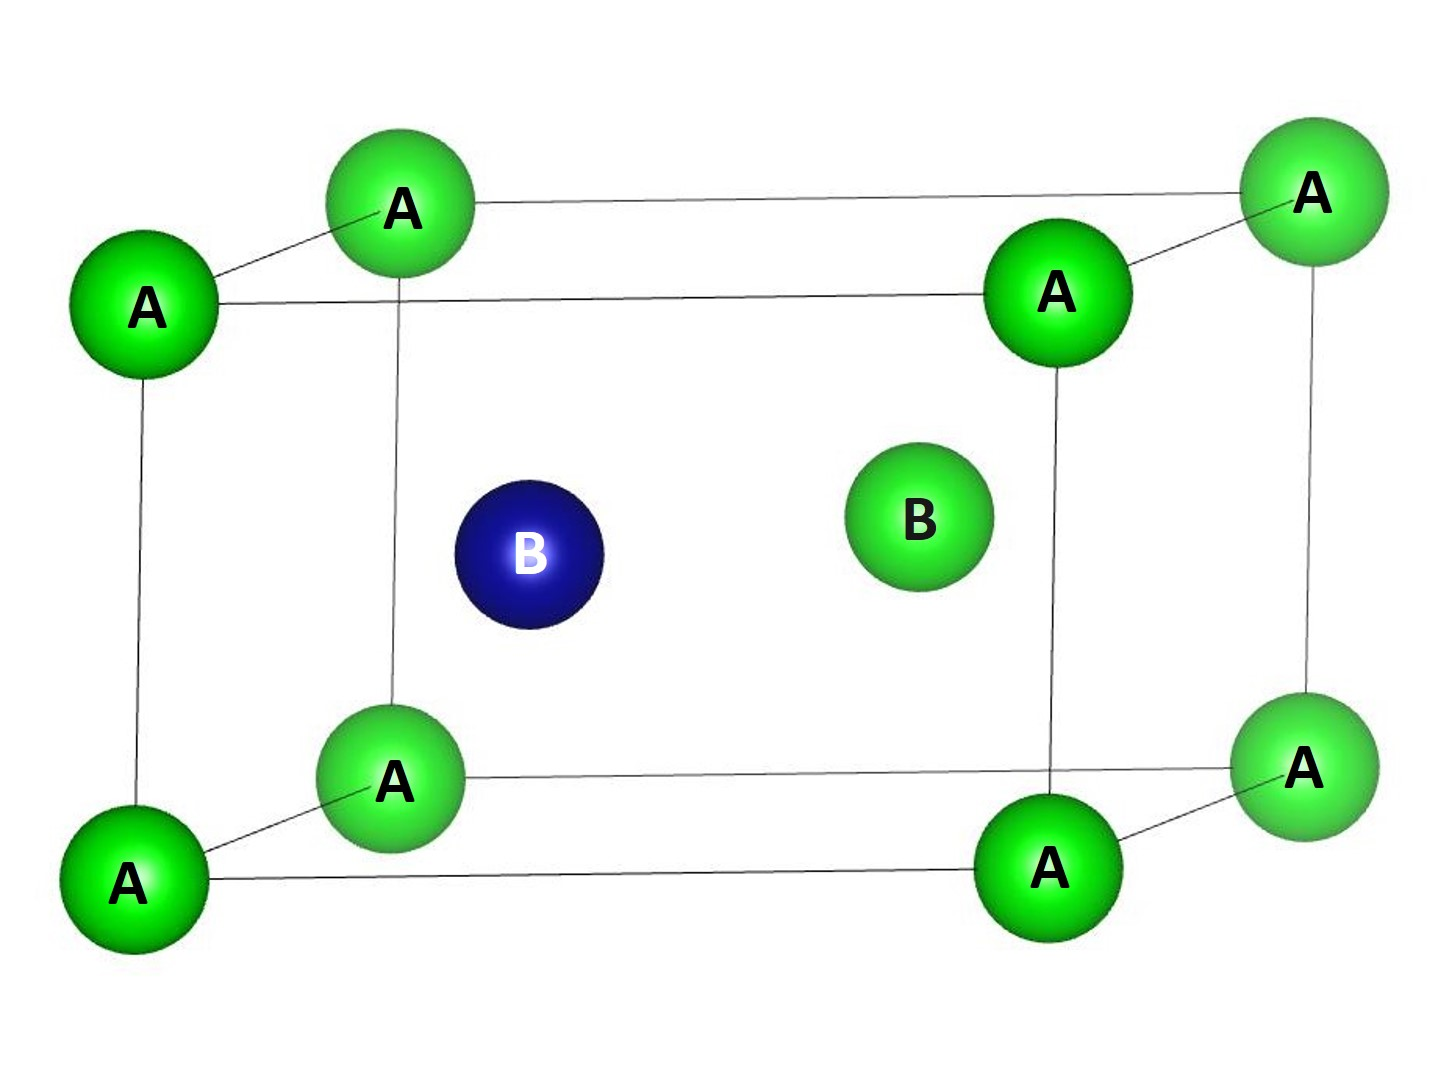
\includegraphics[scale=0.475]{p6mmm_labelled.jpg}
    \caption{The P6/mmm unit cell of the UZr$_2$ structure. The $A$ sites at the corners are always occupied with Zr (green). The $B$ sites at $z=0.5c_0$ are randomly populated with Zr (green) and U (blue).}
    \label{fig:uzr2 structure}
\end{figure}


Density functional theory (DFT) has proven to be an invaluable tool for the exploration of the fundamental structure and properties of crystalline phases  \cite{cohen_challenges_2012, burke_perspective_2012}. However, the difficulties in the DFT analysis of the $\delta$ phase include chemical ordering, magnetism, and the scarcity of experimental data to benchmark. The $\delta$ phase has a hexagonal crystal structure with a space group P6/mmm with a partially ordered structure  \cite{akabori_stability_1992, akabori_lattice_1995}. The A-sites (0,0,0) are mostly occupied with Zr atoms, while U and Zr atoms randomly populate the B-sites (2/3, 1/3, 1/2) and (1/3, 2/3, 1/2) as shown in Figure \ref{fig:uzr2 structure}. $\delta$-UZr$_2$ is paramagnetic according to experiments  \cite{ding_magnetic_2020}. The complexity of modeling paramagnetic ordering in first-principles calculations is addressed in the literature by proposing the dynamic mean field theory (DMFT) method  \cite{anisimov_investigation_2014, abrikosov_recent_2016}. \textit{Ab initio} molecular dynamics (AIMD) had been used to model paramagnetism at finite temperatures as an alternative to the computationally expensive DMFT method  \cite{steneteg_equation_2012}. 
The other difficulty is the scarcity of experimental data on which computational methods may be validated. For instance, we only have a single experimental value of -4.0 $\pm$ 10.1 kJ/mol (-0.014 $\pm$ 0.035 eV/atom) for the formation enthalpy of $\delta$-UZr$_2$ at 298.15 K in the literature. This value was reported by Nagarajan et al. \cite{nagarajan_enthalpy_1993} in a dissolution calorimetry experiment. However, Gyasi et al. \cite{gyasi_about_2022} presented a thorough critique of that experiment and estimated a new endothermic value of 15.5 $\pm$ 17.1 kJ/mol (0.054 $\pm$ 0.059 eV/atom). Both values are questionable and additional measurements are needed to confirm a value for the formation enthalpy of this intermetallic phase. Previously, Ogawa \cite{ogawa_free_1994} commented on the results obtained by Nagarajan et al. \cite{nagarajan_enthalpy_1993} and suggested that the destabilization of $\delta$-UZr$_2$ by nitrogen and oxygen makes it difficult to measure its relative stability without a significant error. That confusion led to adopting a value of zero to the enthalpy of formation of $\delta$-UZr$_2$ in Calphad models \cite{chevalier_progress_2004}. Moreover, other basic properties such as elastic constants of $\delta$-UZr$_2$ are still unmeasured experimentally. Regardless, several DFT studies have attempted to model the $\delta$-UZr$_{2}$ phase \cite{xie_correlation_2013, matar_first_2017, ding_magnetic_2020, ghosh_chemical_2021}. 

Ghosh, et al. \cite{ghosh_chemical_2021} investigated different chemical orderings using special quasirandom structure (SQS) cells of 24 atoms. They reported lattice parameters, enthalpies, and elastic properties for structures with different ordering. However, they did not report the magnetic state of $\delta$-UZr$_2$ in their calculations. Also, their HSE06 hybrid functional results showed a pseudo gap in the density of states which is not physical for this metallic system. Xie, et al. \cite{xie_correlation_2013} employed the DFT+U method on SQS cells of 12 atoms and obtained a theoretical Hubbard U value for $\delta$-UZr$_2$ of 2.21 eV following the linear response approach \cite{cococcioni_linear_2005}. Still, in their calculations, the Hubbard U term was treated as a fitting parameter to the formation enthalpies of U-Zr binary phases, with values between 1 and 1.5 eV resulting in reasonable energetics \cite{xie_correlation_2013}. These values are expected to increase the local magnetic moments, however, Xie et al. \cite{xie_correlation_2013} only reported the total magnetic moments of the simulation cell divided by the total number of atoms including Zr atoms. This may lead to misinterpretation of the reported values because they mention that the moments are mostly on U sites rather than Zr sites, however, they did not report local magnetic moments. They described the local magnetic moments as random and not forming a ferromagnetic or antiferromagnetic ordering. For instance, if we look at the reported spin magnetic moment of the whole simulation cell, we can observe that it increased from 0 to 0.35 Bohr magneton ($\mu_B$) per atom (which implies 1.05 $\mu_B$ per U atom) when adding a Hubbard U of 1.24 eV. This introduced magnetization cannot be ignored and should be of great concern when using DFT+U. The use of the DFT+U method in the treatment of U-Zr systems by Xie et al. \cite{xie_correlation_2013} has been criticized in a comment on that paper by Soderlind et al. \cite{soderlind_comment_2014}. It is argued that the use of the Hubbard U correction leads to unrealistic large volumes and also gives rise to magnetism in non-magnetic systems. In another study, Matar \cite{matar_first_2017} suggested that ferromagnetic ordering is the ground state (energetically more favorable than antiferromagnetic ordering) for $\delta$-UZr$_2$ according to DFT calculations at 0 K, which does not agree with experimental findings. 

In this work, the goal is to investigate $\delta$-UZr$_2$ using first-principles calculations while accurately accounting for the magnetic state. We pursue ordered, partially ordered, and SQS supercells at 0 K and at finite temperatures using AIMD. Both DFT and DFT+U methods will be implemented to explore the effect of the Hubbard U term.

\section{Methodology and Computational Details}

\subsection{Density Functional Theory Calculations}
The projector-augmented wave method (PAW) \cite{blochl_projector_1994} implemented in VASP \cite{kresse_ab_1993,kresse_efficient_1996} was utilized in this work. A cutoff energy of 500 eV is used in all simulations. In 0 K calculations, 3$\times$3$\times$5 and 6$\times$6$\times$2 k-points meshes were applied for the 24-atom ordered and SQS cells, respectively. These meshes were chosen according to a total energy convergence criterion of 1 meV/atom. Meshes of 2$\times$2$\times$4 and 4$\times$2$\times$4 were used for 81-atom (ordered 3$\times$3$\times$3 supercells) and 72-atom (ordered 2$\times$3$\times$4 supercells or SQS cells) systems, respectively. At finite temperatures, a coarser k-point mesh of 2$\times$2$\times$2 was utilized for 81-atom and 72-atom systems to reduce computational expense. The initial AIMD calculations were performed with the 3$\times$3$\times$3 ordered supercell with an initial magnetic moment of zero on all U sites. Then, the choice of 72-atom systems was made to assign an initial antiferromagnetic ordering on an even number of U sites (24 U atoms). These two categories of structures will be referred to as non-magnetic and antiferromagnetic, respectively. However, it should be noted that non-magnetic here does not mean a non-spin polarized calculation. All the results presented in this paper are from spin-polarized calculations but with different initial magnetic moments.
The effect of including spin-orbit coupling in DFT simulations on magnetism, lattice parameters, and enthalpies of formation was previously found to be minimal in $\delta$-UZr$_2$ \cite{xie_correlation_2013, ghosh_chemical_2021}, thus, spin-orbit coupling was not included in this work.

Both the generalized gradient approximation (GGA) \cite{perdew_generalized_1996} and GGA+U methods were used, where Hubbard U values of 1 eV, 1.5 eV, and 2 eV were applied on the uranium $f$-orbitals \cite{dudarev_effect_1997}. The Hubbard U was added using a ramping technique in both 0 K and AIMD calculations. The theoretical Hubbard U values obtained by the linear response approach in the literature for $\alpha$-U and $\delta$-UZr$_2$ are 1.87 eV and 2.21 eV, respectively \cite{xie_correlation_2013}. However, when the formation enthalpy of $\delta$-UZr$_2$ is calculated, the same Hubbard U must be applied in the reference phases. This is done because a comparison cannot be made between the ground state energies of two systems obtained by adding two different values of the Hubbard U to the Kohn-Sham Hamiltonian. Additionally, it has been shown that the application of the Hubbard U value for $\alpha$-U is not necessary to accurately predict structural properties \cite{beeler_first_2010,beeler_first_2013,beeler_determination_2021}. It is important to emphasize that Hubbard U in our study is not a fitting parameter to the formation enthalpy. Although the Hubbard U value that yields the experimental formation enthalpy should also result in reasonable values for other physical properties, such as electronic structure and magnetism as suggested by Wang et al. \cite{wang_oxidation_2006}, that approach is not followed here since experimental data for the $\delta$ phase is scarce and its accuracy has been questioned. The goal is to investigate how the Hubbard U parameter and the chemical ordering affect the structural parameters and the magnetic behavior of $\delta$-UZr$_2$ at 0 K and finite temperatures.

Elastic constants are calculated using 2$\times$2$\times$2 ordered supercells (24-atoms) with antiferromagnetic ordering at 0 K with the finite differences technique. A coarser k-point mesh of 2$\times$2$\times$4 was utilized for computational purposes. 



\subsection{Structure Optimization}


The unit cell of $\delta$-UZr$_2$ is shown in Fig. \ref{fig:uzr2 structure}. Our initial study using 0 K DFT involved using 4 different configurations in 24-atom supercells. We fixed the occupancy of the A-site (0,0,0) to be solely occupied by Zr in all of these calculations.
The four structures considered are (1) an ordered 2$\times$2$\times$2 supercell constructed by 8 unit cells with the same chemical ordering; (2) a special quasirandom structure (SQS) cell with a Zr occupancy of 1 at (0,0,0) and with an occupancy of 0.5 for both Zr and U at the other two sites; (3) an ordered supercell as (1) but with switching the Zr and U in B-sites positions in only one of the 8 unit cells; and (4) a 2$\times$2$\times$2 supercell with 4 unit cells having an alternating occupancy at B-sites. Complete compositionally disordered UZr$_2$ is believed to be a metastable structure called the $\omega$ phase that exists during cooling from the $\gamma$ phase to the low-temperature $\delta$ phase. It was also observed in quenched and as-cast U-Zr alloys \cite{irukuvarghula_decomposition_2016}. However, that phase is beyond the scope of this work. SQS cells were constructed with the ATAT code\cite{van_de_walle_alloy_2002,van_de_walle_multicomponent_2009,van_de_walle_efficient_2013}. 

Final 0 K calculations were made after equilibrating these structures at 100 K with AIMD. The initialization of atomic positions for 0 K structural relaxation calculations is obtained from the 100 K equilibrated structure. This facilitated the ionic relaxation at 0 K and was observed to be necessary to yield non-magnetic and antiferromagnetic structures with lower energies than the initially obtained ferromagnetic structure, as will be shown. 

\subsection{\textit{ab initio} Molecular Dynamics}

The AIMD simulations on UZr$_2$ were performed using an NPT ensemble with a Langevin thermostat and a timestep of 2 fs. First, an equilibration run of at least 1000 timesteps (2 picoseconds) was performed.   Then, production runs were performed for a minimum of 2000 timesteps (4 picoseconds) for each temperature in the range of 100 K to 600 K with an increment of 100 K to calculate thermal expansion and heat capacities. Temperature ramping was used to reduce the equilibration time required prior to each production run. The same procedure was followed with pure $\alpha$-U and $\alpha$-Zr systems. A 108-atom supercell was used to model the $\alpha$-U reference phase with a 2$\times$1$\times$1 k-points mesh, while a 96-atom supercell was used for the $\alpha$-Zr phase with a 2$\times$2$\times$2 k-points mesh. The potential energies ($E_0$) of each of the three systems were time-averaged to calculate the enthalpies of formation ($\Delta H$) at finite temperatures according to the following equation:
\[\Delta H = E_0(\delta UZr_2) - E_0(\alpha U) - E_0(\alpha Zr) \]
and the time-averaged total energies ($E$) of $\delta$-UZr$_2$ were used to calculate the heat capacities (C$_p$) as follows:
\[C_p(T) = \frac{E(T+\Delta T) - E(T-\Delta T)}{2 \Delta T} \]
Finally, the linear thermal expansion coefficient is obtained from the slope of the time-averaged lattice parameters $a$ and $c$ in the ordered supercells when plotted versus temperature.
%{\color{red}
%How do you define thermal expansion? Where is the reference state? Or is it the slope of the full system? Provide the equation for the heat capacity and the enthalpy of mixing. Does anything else need to be included? I want us to be complete.
%}

\section{Results}

\subsection{Structural Relaxation: From 0 K to Finite Temperature}

Initial 0 K calculations resulted in a ferromagnetic ground state when using either GGA or GGA+U methods. A non-magnetic or anti-ferromagnetic state was not achieved for any system via the typical DFT relaxation. Reasonable accuracy was obtained for the atomic volume for U values of 2 eV and below, but a negative formation enthalpy was only achieved at Hubbard U = 3 eV and 4 eV for ferromagnetic $\delta$-UZr$_2$. However, the atomic volume was highly overestimated using that setup. At U = 3 eV, the volume per atom was between 24.51 and 24.68 {\AA}$^3$/atom, depending upon the configuration. While at U = 4 eV, values between 24.84 and 24.98 {\AA}$^3$/atom were obtained. For reference, the experimental volume per atom is reported to be 22.58 {\AA}$^3$ at room temperature \cite{akabori_lattice_1995}. Moreover, ionic relaxation difficulties arise when applying these high U values on the $f$-orbital in the pure $\alpha$-U phase which is a reference in calculating the enthalpy of formation.

Subsequently, systems were equilibrated at 100 K utilizing AIMD for 4 ps. As stated, this equilibrated structure is utilized as the starting point for ionic relaxations at 0 K. Using a non-magnetic initialization for the ordered 3$\times$3$\times$3 supercell, the optimized structure was non-magnetic and more stable by 0.1 eV/atom compared to the ferromagnetic structure obtained by GGA prior to AIMD equilibration. The AIMD equilibrated structures are approximately 1\% lower in volume (22.39 {\AA}\textsuperscript{3}/atom versus 22.66 {\AA}\textsuperscript{3}/atom) compared to the initial 0 K relaxation. % as shown in Table \ref{tab:V_H_pre_eq}. 


Following the same approach, assigning antiferromagnetic ordering to the 72-atom ordered and SQS cells yielded an even more stable configuration with lower energy. We believe that these antiferromagnetic structures are the ground state of UZr$_2$ according to GGA. This process and these findings have been observed for other uranium compounds, such as UN \cite{kocevski_finite_2023}, where a non-zero temperature simulation was required to obtain the appropriate ground state magnetic ordering and more accurate electronic and thermal properties. Thus, it is emphasized that it appears to be required to utilize an initial AIMD simulation to reach the true 0 K ground state configuration and magnetic state for some uranium compounds. 

In addition to changes in the volume/energy, there are associated changes in local bond structure which allow for the convergence to a non-magnetic or anti-ferromagnetic state. In the ordered structure, the change is most apparent from an analysis of the radial distribution function. There is a single U-U peak at 3.1 {\AA} in the idealized 0 K pre-equilibration structure. After AIMD relaxation, that single peak splits into two peaks at distances of 2.5 and 3.8 {\AA}. What this physically corresponds to is U atoms alternately moving up or down in the $c$-axis. In the SQS structure, the equilibration process results in a minimally shorter U-U distance.

%more dramatic such that the U-U distances along the $c$-axis change from 3.1 {\AA} to 3.5 {\AA} and 3.8 {\AA}, alternatively, breaking the symmetry of the cell.



\begin{comment}
\begin{table}[ht!]
    \centering
    \caption{Volume (V) and enthalpies of formation ($\Delta$H) per atom for ordered and SQS supercells before equilibration with ferromagnetic (FM) ordering, and after equilibration with nonmagnetic (NM) and antiferromagnetic (AFM) ordering. These values are obtained using GGA (Hubbard U = 0)}
    \label{tab:V_H_pre_eq}
    \begin{tabular}{|c|c|c|c|c| }
    \hline
    &   Ordered & SQS \\
    \hline
    & V (\AA$^3$/atom) | $\Delta$H (eV/atom) &   V (\AA$^3$/atom) | $\Delta$H (eV/atom) \\
    \hline
    Pre-equilibration (FM) & 22.66  | 0.18 & 22.68 | 0.14 \\
    \hline
    Post-equilibration (NM) & 22.39 | 0.11 & 22.48 | 0.09 \\
      \hline
    Post-equilibration (AFM) & 22.78 | 0.07 & 22.49 | 0.09 \\
      \hline
    \end{tabular}
\end{table}
\end{comment}

A note should be included regarding the alternate structures explored. The structure identified as number (4) consistently displays higher energy than either the ordered or SQS structures. The structure identified as number (3) has sublattice disordering such that it is impossible to converge to an antiferromagnetic state. Thus, only the ordered and SQS supercells are utilized for the remainder of the work presented. 

\subsection{Structure and Thermophysical Properties}

The formation enthalpy and the atomic volume of the optimized structures of the ordered and the SQS cell are shown in Figure \ref{fig:1} for temperatures between 0 K and 600 K. It should be noted that this graph includes the $quenched$ 0 K DFT data and results from full AIMD simulations at non-zero temperatures. Both GGA and GGA+U results are presented for Hubbard U values of 1 eV, 1.5 eV, and 2 eV. Unless labeled otherwise, all of the results reported are of the antiferromagnetic structures. It can be observed that the enthalpy of formation is almost temperature-independent below 600 K. The average enthalpy of formation of a formula unit of $\delta$-UZr$_2$ from pure GGA (without using Hubbard U) is 0.252 eV (0.084 eV/atom) and 0.233 eV (0.078 eV/atom) for the SQS and ordered supercells, respectively. The only experimental measurement reported in the literature is -0.04 eV per formula unit (-0.014 eV/atom) \cite{nagarajan_enthalpy_1993}. Although we expect a negative enthalpy because this phase is stable at low temperatures, the accuracy of that single measurement is questionable as suggested recently by Gyasi et al. \cite{gyasi_about_2022}, whose modified value is also included in Fig. \ref{fig:1}a. The GGA+U method brought the formation enthalpies closer to the experimental value, and at U = 2 eV a negative formation enthalpy was achieved. However, the GGA+U method leads to an overestimation of the atomic volume by approximately 6\%, as seen in Fig. \ref{fig:1}b, which is considered a large discrepancy. This observation was noted before by Soderlind et al. \cite{soderlind_comment_2014} in their comment on the results from Xie et al. \cite{xie_correlation_2013} using GGA+U.

\begin{figure}[h!]
    \centering
    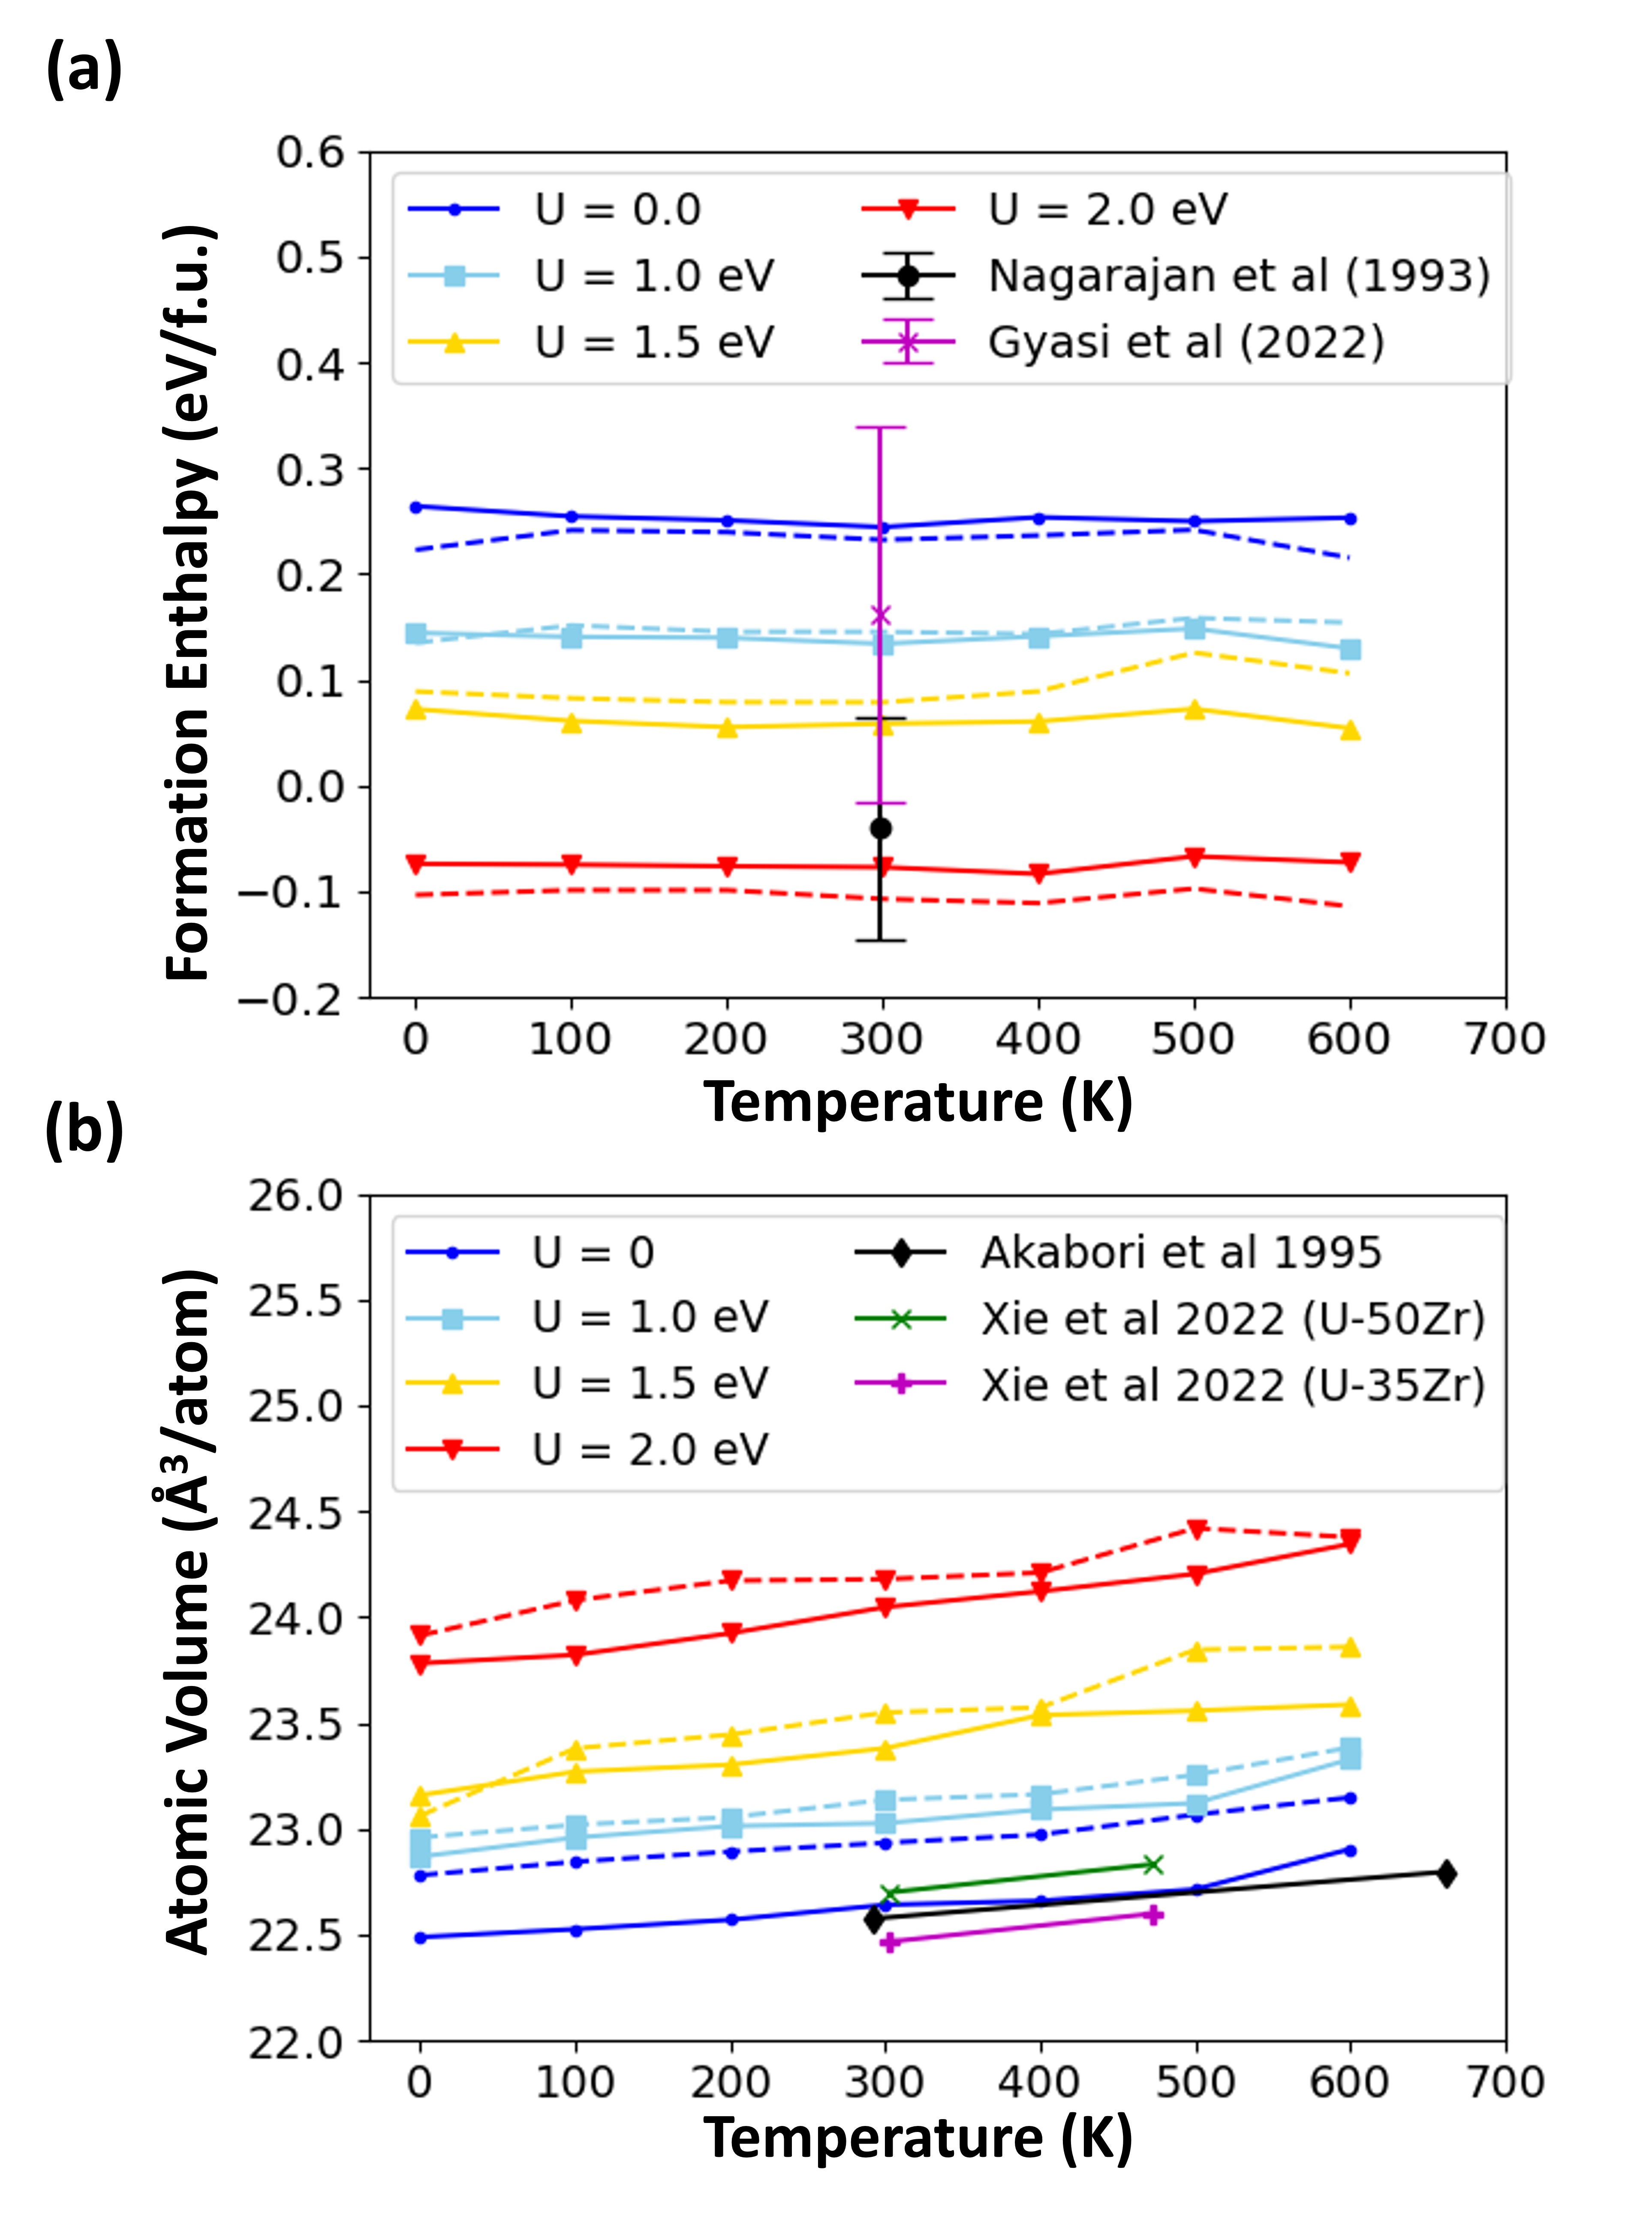
\includegraphics[width=0.75\textwidth]{H__Vol.jpg}
    \caption{(a) The enthalpy of formation per formula unit of $\delta$-UZr$_2$ obtained from SQS (solid lines) and ordered cells (dashed lines); (b) The atomic volume versus temperature of SQS cells (solid), and ordered supercells (dashed). The experimental values are from references \cite{akabori_lattice_1995, nagarajan_enthalpy_1993,xie_phase_2022, gyasi_about_2022}.}
    \label{fig:1}
\end{figure}

The atomic volumes obtained using Hubbard U values of 0, 1, 1.5, and 2 eV are plotted in Figure \ref{fig:1}b. It can be observed that GGA results (U = 0) are in good agreement with experiments \cite{akabori_lattice_1995, xie_phase_2022}, with the SQS structure exhibiting a near exact match to experimental results. The atomic volume increases and deviates from the experimentally measured value by increasing the value of the Hubbard U. Thus, one is not able to simultaneously achieve an optimized volume that favorably compares to experiment while also obtaining a negative formation enthalpy. Increasing the magnitude of on-site Coulombic repulsion increases the volume while decreasing the formation enthalpy. 


The associated lattice parameters and atomic volume of the optimized structures at 0 K and room temperature are shown in Table \ref{tab: cell parameters} for both non-magnetic and AFM states. Although the perfectly-ordered supercells (O-NM and O-AFM) do not represent the true partially-ordered UZr$_2$ observed experimentally, they allow us to calculate the lattice parameters $a$ and $c$, unlike the SQS cells. The a$_1$ and a$_2$ lattice parameters in the ordered supercells are not identical because the optimized supercells broke the hexagonal symmetry, thus we report an average value for the lattice parameter $a$ to compare with experiments. The values after the $\pm$ sign in Table \ref{tab: cell parameters} represent the standard deviation of this lattice parameter. We observe a 2 \% increase of lattice parameter $c$ when changing the magnetic ordering from the non-magnetic to the antiferromagnetic structure, which is likely the source of the overestimation of the atomic volume in the antiferromagnetic ordered supercells as reported in Table \ref{tab: cell parameters} and Figure \ref{fig:1}. However, it should be restated that the antiferromagnetic ordered cells had an energy approximately 35 meV/atom lower than the non-magnetic ordered supercells. On the other hand, the atomic volume of the SQS cell has very good agreement with experimental values \cite{akabori_lattice_1995, xie_phase_2022}, but extracting information about the lattice parameters from this system is not applicable.
%Here, we emphasize that tuning 
\begin{table}[h!]
    \centering
    \caption{Lattice parameters and volume per atom at 0 K and room temperature calculated by GGA (U = 0) for non-magnetic and antiferromagnetic perfectly-ordered supercells (O-NM and O-AFM, respectively), and for antiferromagnetic SQS cells (SQS-AFM). Data are compared against room temperature experiments \cite{xie_phase_2022,akabori_lattice_1995}.} 
    \begin{tabular}{|c|c|c|c|c|c|c| }
    \hline
T &  &a (\AA)  & c (\AA) & V/atom (\AA$^3$)  \\
 \hline
       & O-NM   & 5.026 $\pm$ 0.003  &3.073 & 22.39\\
      0 K     & O-AFM      &  5.004 $\pm$ 0.004  & 3.145 & 22.78\\
   &  SQS-AFM       &  - & - & 22.49\\
   \hline
  &  O-NM   & 5.043  $\pm$ 0.002 &   3.083&  22.58 \\
                         &   O-AFM   & 5.020 $\pm$ 0.005  & 3.147 &  22.93 \\
                          &   SQS-AFM  &  -  & -   & 22.64  \\
       Room Temp.                     & U-50Zr (72 at.{\%} Zr) \cite{xie_phase_2022}  & 5.040   &3.096  & 22.70  \\
             & U-35Zr (58 at.{\%} Zr)  \cite{xie_phase_2022}  & 5.028   &3.077  &22.47   \\
                          & U-48Zr (71 at.{\%} Zr) \cite{akabori_lattice_1995} &5.032   &3.089  &  22.58\\
     \hline
    \end{tabular}
    \label{tab: cell parameters}
\end{table}


\begin{figure}[h!]
     \centering
    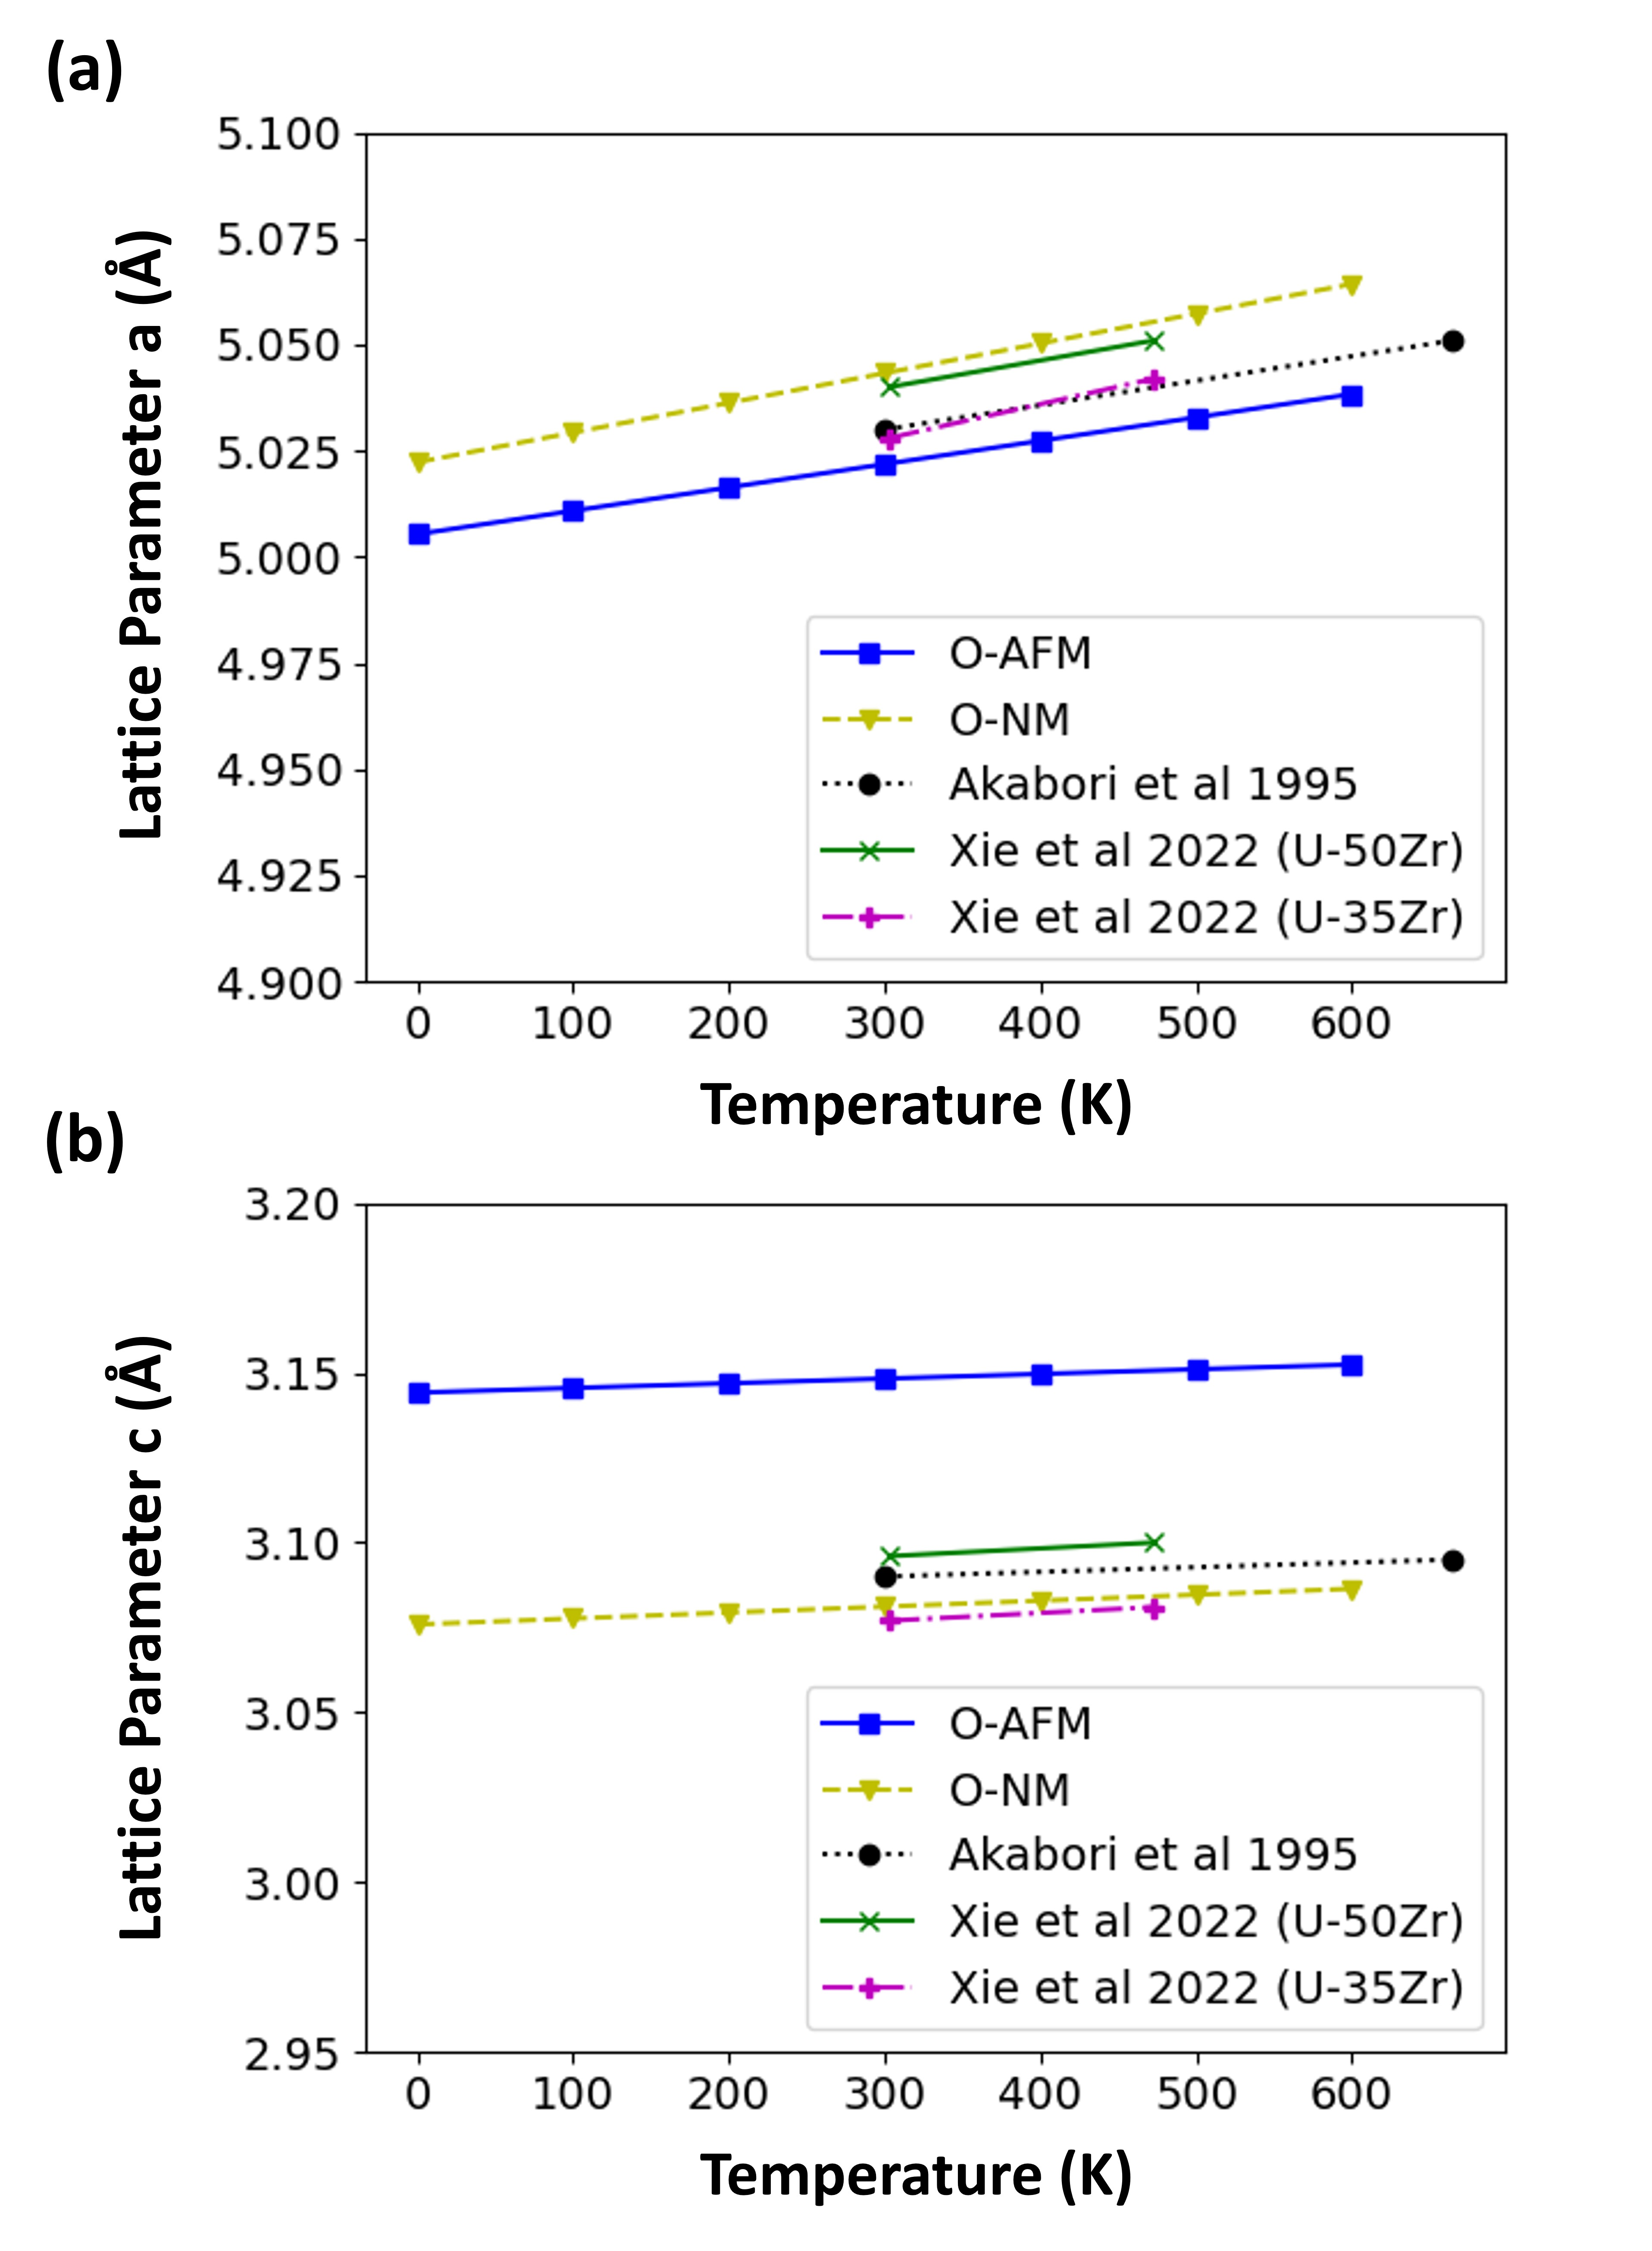
\includegraphics[scale=0.2]{cell_parameters.jpg}
    \caption{The average lattice parameter $a$ in panel (a) and lattice parameter $c$ in panel (b) versus temperature from GGA calculations in the ordered supercell for the antiferromagnetic (AFM) and the non-magnetic (NM) structures. The experimental values are from references  \cite{akabori_lattice_1995} and \cite{xie_phase_2022}.
    \label{fig lat_par}}
\end{figure}

The thermal expansion behavior in UZr$_2$ can be observed in Figure \ref{fig:1} as the slope of the volume with respect to temperature. Qualitatively, the volumetric thermal expansion of both the ordered and SQS cells according to GGA (U=0) are close to experiments \cite{akabori_lattice_1995, xie_phase_2022}. But to have a closer quantitative look at the anisotropy of the thermal expansion, we plot the lattice parameters $a$ and $c$ from the ordered supercells versus temperature in Figure \ref{fig lat_par}. The thermal expansion coefficient (the slope in the figure) in the ordered supercell agrees well with experiments in the literature despite the slight differences in the absolute values of $a$ and $c$. The temperature evolution of the lattice parameters $a$ and $c$
in the AIMD simulations can be described by a linear relation for the non-magnetic supercell as follows: 

\[
 a(T) = 5.02 + 7.00 \times 10^{-5} T \]
 \[
 c(T) = 3.07 + 1.75 \times 10^{-5} T \]

\noindent and, for the antiferromagnetic (AFM) supercell as follows:
\[
 a(T) = 5.00 + 5.50 \times 10^{-5} T \]
 \[
 c(T) = 3.14 + 1.38 \times 10^{-5} T \]
 The experimental temperature evolution of the lattice parameters according to Xie et al. \cite{xie_phase_2022} is:

 \[
 a(T) = 5.002 + 8.384 \times 10^{-5} T \]
 \[
 c(T) = 3.076 + 0.996 \times 10^{-5} T \]

These equations translate into a thermal expansion coefficient of the $a$ lattice parameter of $1.4 \times 10^{-5}$ and $1.1 \times 10^{-5}$ in the NM and the AFM supercells, respectively, while the thermal expansion coefficient of the $c$ lattice parameter is $5.7 \times 10^{-6}$ and $4.4 \times 10^{-6}$ in the NM and the AFM supercells, respectively. The experimental values reported by Xie and coworkers are $1.66 \times 10^{-5}$   and  $3.2 \times 10^{-6}$  for the lattice parameters $a$ and $c$, respectively. The agreement in the expansion coefficient in both the $a$ and $c$ directions for both magnetic configurations is considered reasonable to excellent. A more recent experiment on the thermal evolution of the U-Zr system used a second-order polynomial fit to describe the thermal expansion behavior \cite{williams_phase_2023}. That approach yields a temperature-dependent thermal expansion coefficient. For the $\delta$-UZr$_2$ in a U-30Zr casting, Williams and coworkers \cite{williams_phase_2023} report coefficients of thermal expansion of $7.7 \times 10^{-9} T + 1.34 \times 10^{-5}$ and $-1.46 \times 10^{-8} T + 1.05 \times 10^{-5}$ for $a$ and $c$  lattice parameters, respectively. Our computed coefficients of thermal expansion are also in reasonable agreement with this experiment for temperatures below 600 K. 

%\FloatBarrier 

We also computed the heat capacities at constant pressure from the AIMD total energies, and our results are compared with experiments \cite{takahashi_heat_1989, ding_magnetic_2020} in Figure \ref{fig:2}. The agreement of our heat capacities calculated using antiferromagnetic structures with experiments \cite{takahashi_heat_1989} is excellent. This is in contrast to the non-magnetic structure as observed in Figure \ref{fig:2}, which drastically overestimates the heat capacity. This result provides confidence in the choice of antiferromagnetic ordering to model the paramagnetic UZr$_2$. Moreover, we found that the calculated heat capacities do not depend on the Hubbard U value for the AFM state, as shown in Figure \ref{fig:heat_cap_afm}. 
%thus there remains a lack of evidence to justify the utilization of a Hubbard U term for the description of UZr$_2$. 

\begin{figure*}[h!]
    \centering
    \begin{subfigure}[]{0.48\textwidth}
    \centering
    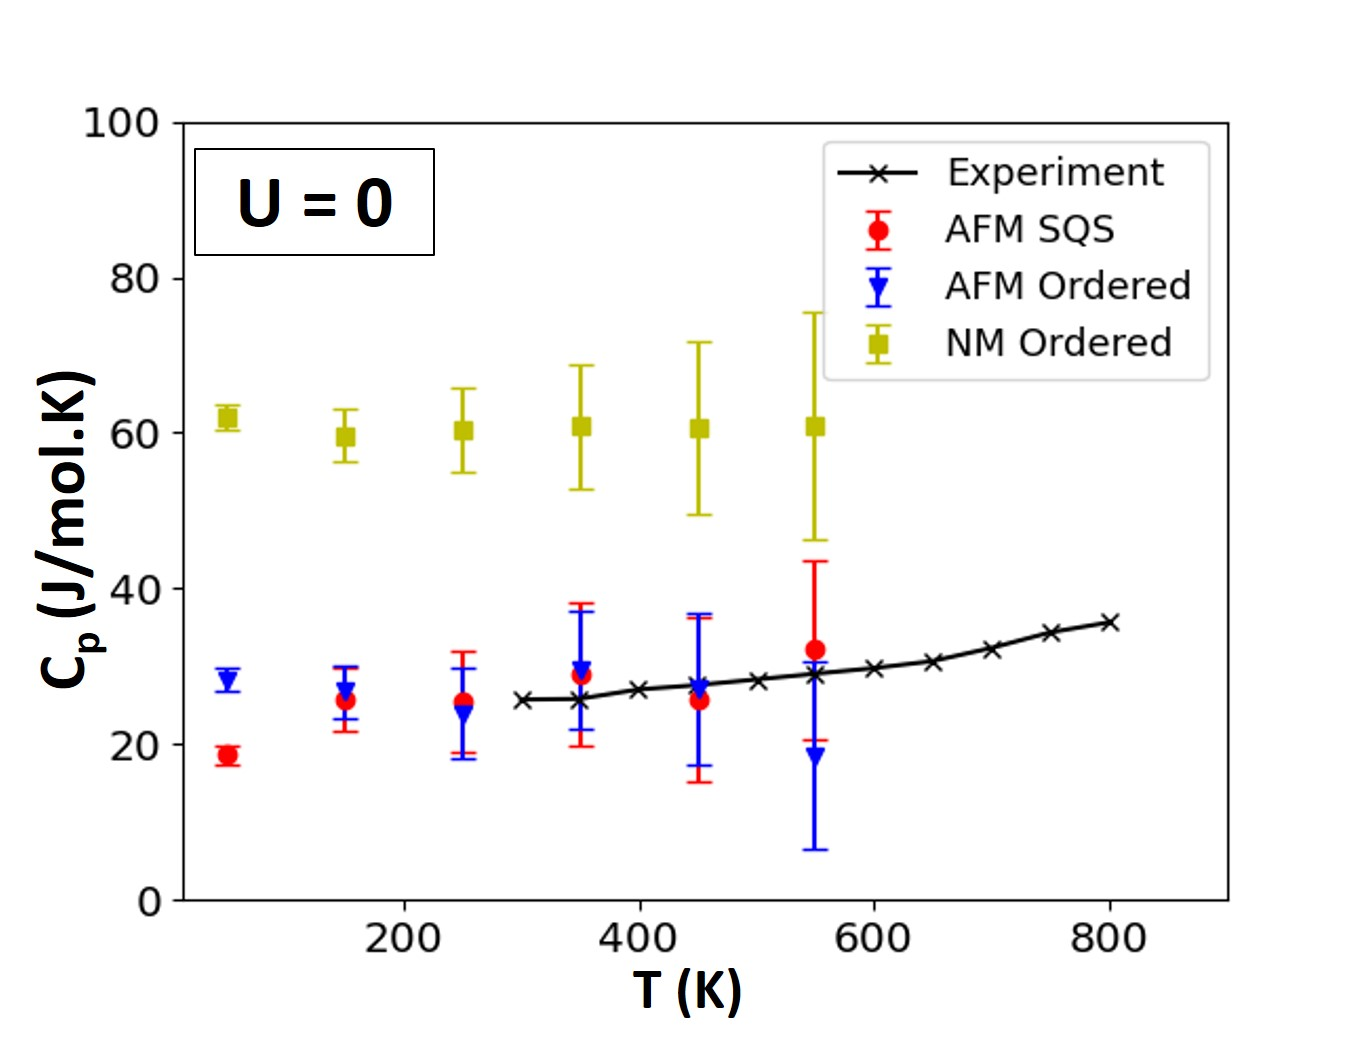
\includegraphics[width=\textwidth]{cp_u0.jpg}
    \caption{}
    \label{fig:2}
    \end{subfigure}
    ~
    \begin{subfigure}[]{0.48\textwidth}
    \centering
    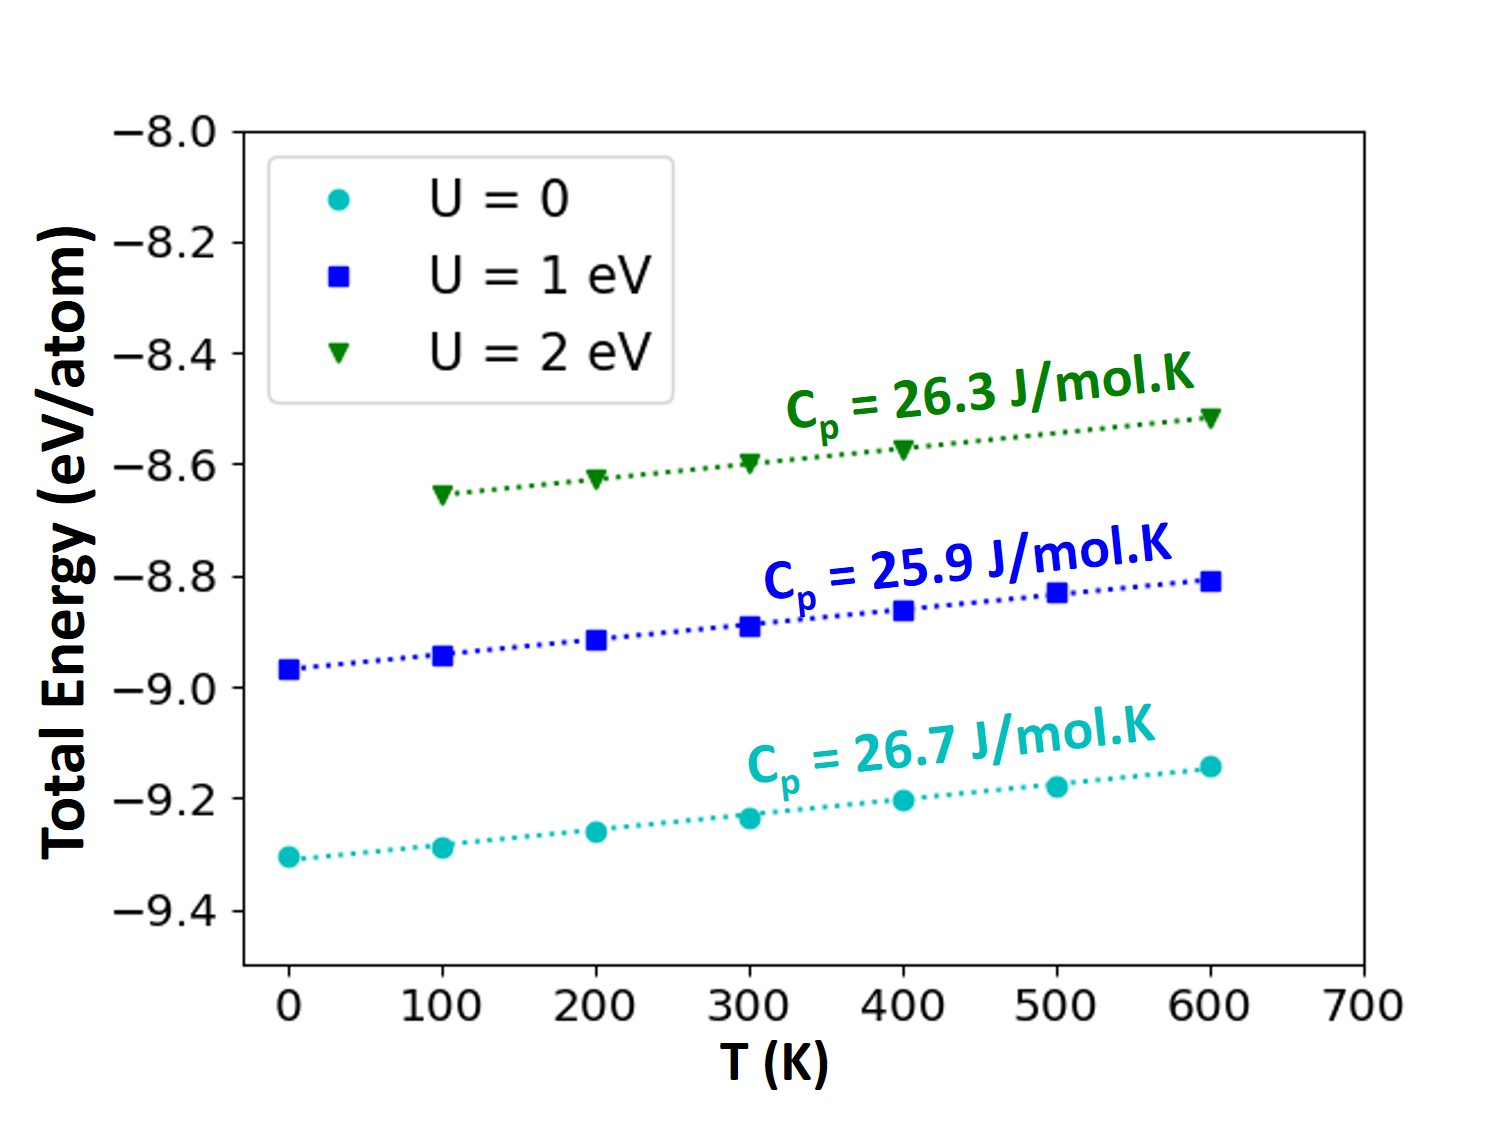
\includegraphics[width=\textwidth]{etot_sqs.jpg}
    \caption{}
    \label{fig:heat_cap_afm}
\end{subfigure}
    \caption{a) The calculated heat capacities versus temperature from antiferromagnetic (AFM) cells and non-magnetic (NM) ordered supercells using GGA (U = 0). The experimental values are from reference \cite{takahashi_heat_1989}. b) The constant heat capacity calculated from the slope of total energy versus temperature in antiferromagnetic (AFM) SQS cells. }
\end{figure*}

Finally, elastic constants were calculated using the finite-differences approach as implemented in VASP for the AFM ordered 2$\times$2$\times$2 supercell, and the results are shown in Table \ref{tab:elas_const}. Experimental measurements of the elastic constants of this phase are not available up to the date of publishing this paper. So, the elastic constants of the pure $\alpha$-U and $\alpha$-Zr phases are shown in Table \ref{tab:elas_const} for comparison. The computationally calculated elastic constants by Ghosh et al. \cite{ghosh_chemical_2021} for an ordered supercell are also included in the table. An asymmetry can be observed in the C$_{11}$ and C$_{22}$ terms although the cell vectors a$_{1}$ and a$_{2}$ are almost identical at 0 K. This reinforces the local disordering of bond lengths that was achieved via thermal equilibration and quenching. Generally, minor differences are observed for the elastic constants affected by the broken symmetry (C$_{11}$ and C$_{22}$, C$_{13}$ and C$_{23}$, and C$_{44}$ and C$_{55}$). The results show distinct differences from the calculations of Ghosh, namely a factor of two reduction in C$_{33}$ and C$_{13}$/C$_{23}$. The other primary elastic constants, C$_{11}$/C$_{22}$, are also lower than found by Ghosh \cite{ghosh_chemical_2021} by approximately 25 GPa. 

\begin{table}[h!]
    \centering
        \caption{Elastic moduli in GPa calculated from the ordered supercell of $\delta$-UZr$_2$ using 0 K GGA are compared against previous DFT calculations \cite{ghosh_chemical_2021}, and experimental elastic moduli of $\alpha$-Zr measured at 4 K \cite{fisher_single-crystal_1964} and $\alpha$-U measured at room temperature \cite{fisher_adiabatic_1958}.}
    \label{tab:elas_const}
    \begin{tabular}{|c|c|c|c|c|c|c|c|c|c|}
    \hline
Phase & C$_{11}$ & C$_{22}$ & C$_{33}$  & C$_{12}$ & C$_{13}$ & C$_{23}$ & C$_{44}$ & C$_{55}$ & C$_{66}$   \\
 \hline
   $\delta$-UZr$_2$ (This work) &136& 140 & 93 & 64 & 23 &26 & 38 & 39 & 40 \\
   \hline
     $\delta$-UZr$_2$ \cite{ghosh_chemical_2021} &175& 175 & 186 & 92 & 50 &50 & 43 & 43 & 41 \\
   \hline
   $\alpha$-Zr  \cite{fisher_single-crystal_1964} & 155.4 &155.4 &172.5 &67.2 &64.6 &64.6 &36.3 &36.3 &44.1 \\
   \hline
    $\alpha$-U \cite{fisher_adiabatic_1958} & 215&199 &267 &46 &22 &108 & 124& 73&74\\
     \hline
    \end{tabular}
\end{table}

\FloatBarrier

\subsection{Magnetic and Electronic Properties}

The lattice parameters and enthalpies of formation can be modified by changing the on-site Coulomb term (Hubbard U) value which may yield seemingly good results but does not solve the problem of describing the magnetic ordering. Liu and coworkers \cite{liu_choosing_2019} addressed the same problem in the U$_3$Si$_2$ system. We can conclude from their findings that the choice of the magnetic state should precede choosing the Hubbard U value. Supplying the DFT code with a Hubbard U parameter fitted to reproduce a physical property and waiting for the simulations to predict the true magnetic state is highly unlikely to occur, as it strongly depends on the initialization of magnetic moments. In our case, we argue that Hubbard U is not just unnecessary but it also introduces unphysical strong spin polarization, as will be shown in this subsection.

To quantify the degree of spin-polarization, we extracted the local magnetic moment on U sites at 0 K (see Table \ref{tab:mag_AFM_0K}) and the time-averaged local magnetic moments at finite temperature (see Figure \ref{fig:4}). It should be noted that the reported values here are the absolute values regardless of the spin state (up or down). The total net magnetic moments in these AFM structures are very close to zero and are not plotted here.

\begin{figure}[h!]
    \centering
    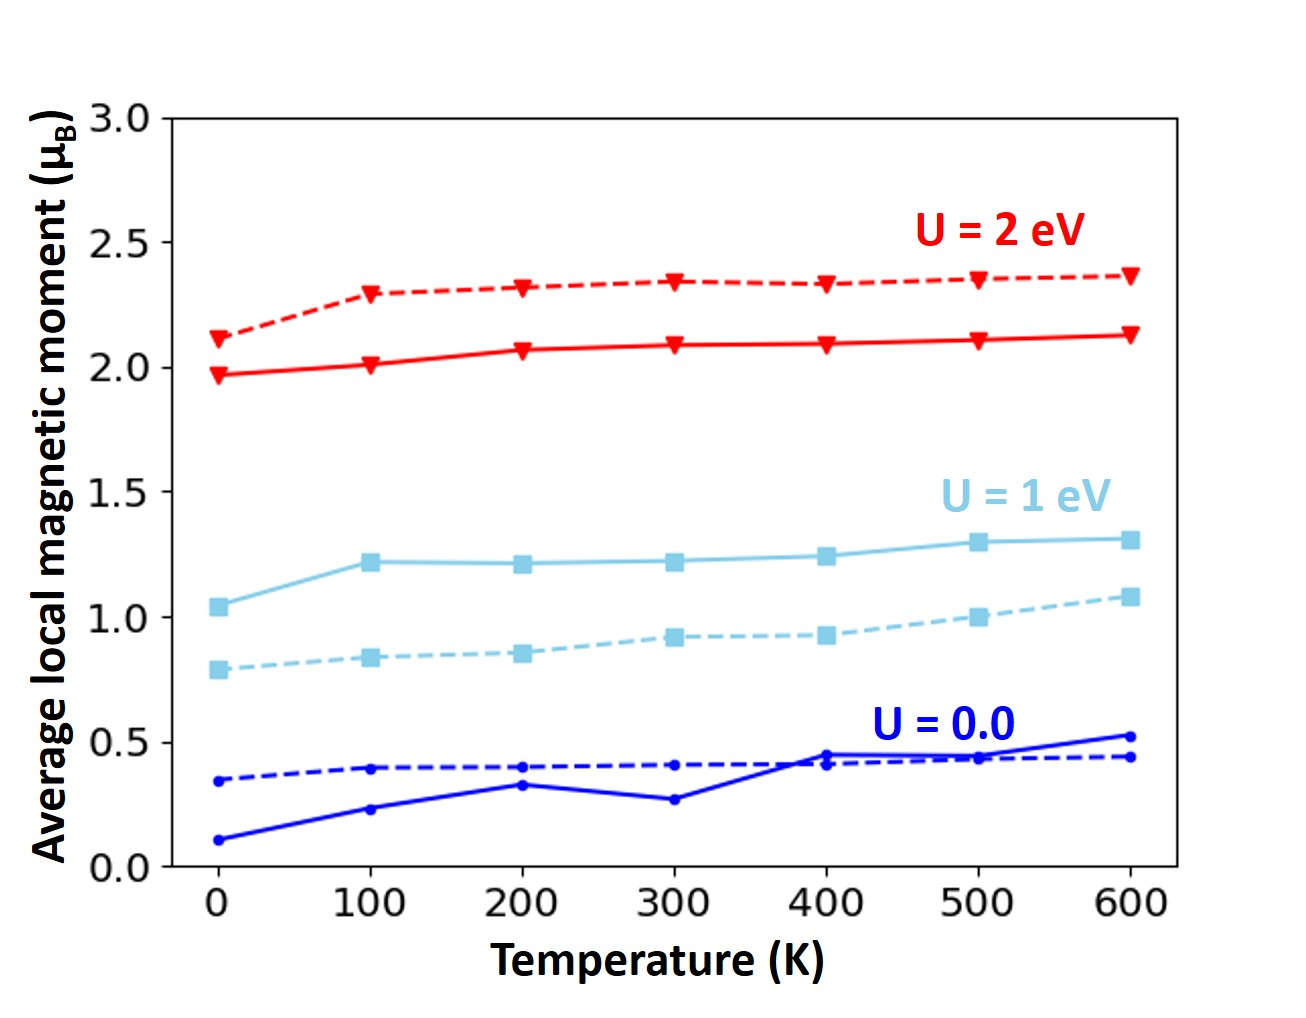
\includegraphics[scale=0.5]{magmom.jpg}
    \caption{The average local magnetic moments on U atoms in antiferromagnetic cells. Solid lines are for SQS cells while dashed lines are for ordered supercells}
    \label{fig:4}
\end{figure}

\begin{table}[h!]
    \centering
    \caption{Local magnetic moment per U atom in antiferromagnetic cells at 0 K}
    \label{tab:mag_AFM_0K}
    \begin{tabular}{|c|c|c| }
    \hline
U(eV) & ($\mu_B$/atom) in O-cell & ($\mu_B$/atom) in SQS   \\
 \hline
      0     &   0.345   &  0.104 \\
 0.5        &       0.600   &    0.738      \\
  1.0 &   0.786      &   1.042 \\
    1.5 & 1.000      &   1.297 \\
    2.0  &      2.110            &      1.965         \\
     \hline
    \end{tabular}
\end{table}

As shown in Figure \ref{fig:4} and Table \ref{tab:mag_AFM_0K}, an increase in Hubbard U increases the local magnetic moments making the UZr$_2$ a perfectly AFM material with full spin polarization of $f$-electrons at U = 2 eV. The reason for that may be an unphysical over-localization of $f$-electrons in a metallic system induced by the Hubbard U. These trends are independent of input atomic structure (SQS versus ordered supercell) or temperature. Although we could not exactly reproduce the paramagnetic state using standard DFT techniques, we argue that the weak antiferromagnetism produced by pure GGA results is the closest to a paramagnetic structure. As a result of this, in conjunction with the other observed thermophysical properties reported here, we suggest using the pure GGA without the Hubbard U correction for the $\delta$-UZr$_2$ phase. 

The electronic density of states (DOS) calculated by GGA and GGA+U are shown in Figure \ref{fig:5}. The DOS from the ordered and the SQS cell in panels $a$ and $b$, respectively, have similar trends but the SQS cell has a smoother DOS. This can be attributed to the random arrangement of atoms. The effect of a U value of 1.5 eV is minimal. The uranium $f$-states are slightly pushed to the right due to the introduced Coulomb term on this orbital. The pseudogap at the Fermi level was observed in a previous DFT study by Ghosh et al. \cite{ghosh_chemical_2021} using both GGA and hybrid functionals. This shape of the DOS is in contradiction with the earlier study in the literature by Xie et al. \cite{xie_correlation_2013} in which the DOS of UZr$_2$ appeared flat around the Fermi level. The agreement with Ghosh et al. provided confidence in the reported values, but unfortunately, no experimental data exist for comparison to truly validate the calculated DOS. 


\begin{figure}[h!]
    \centering
    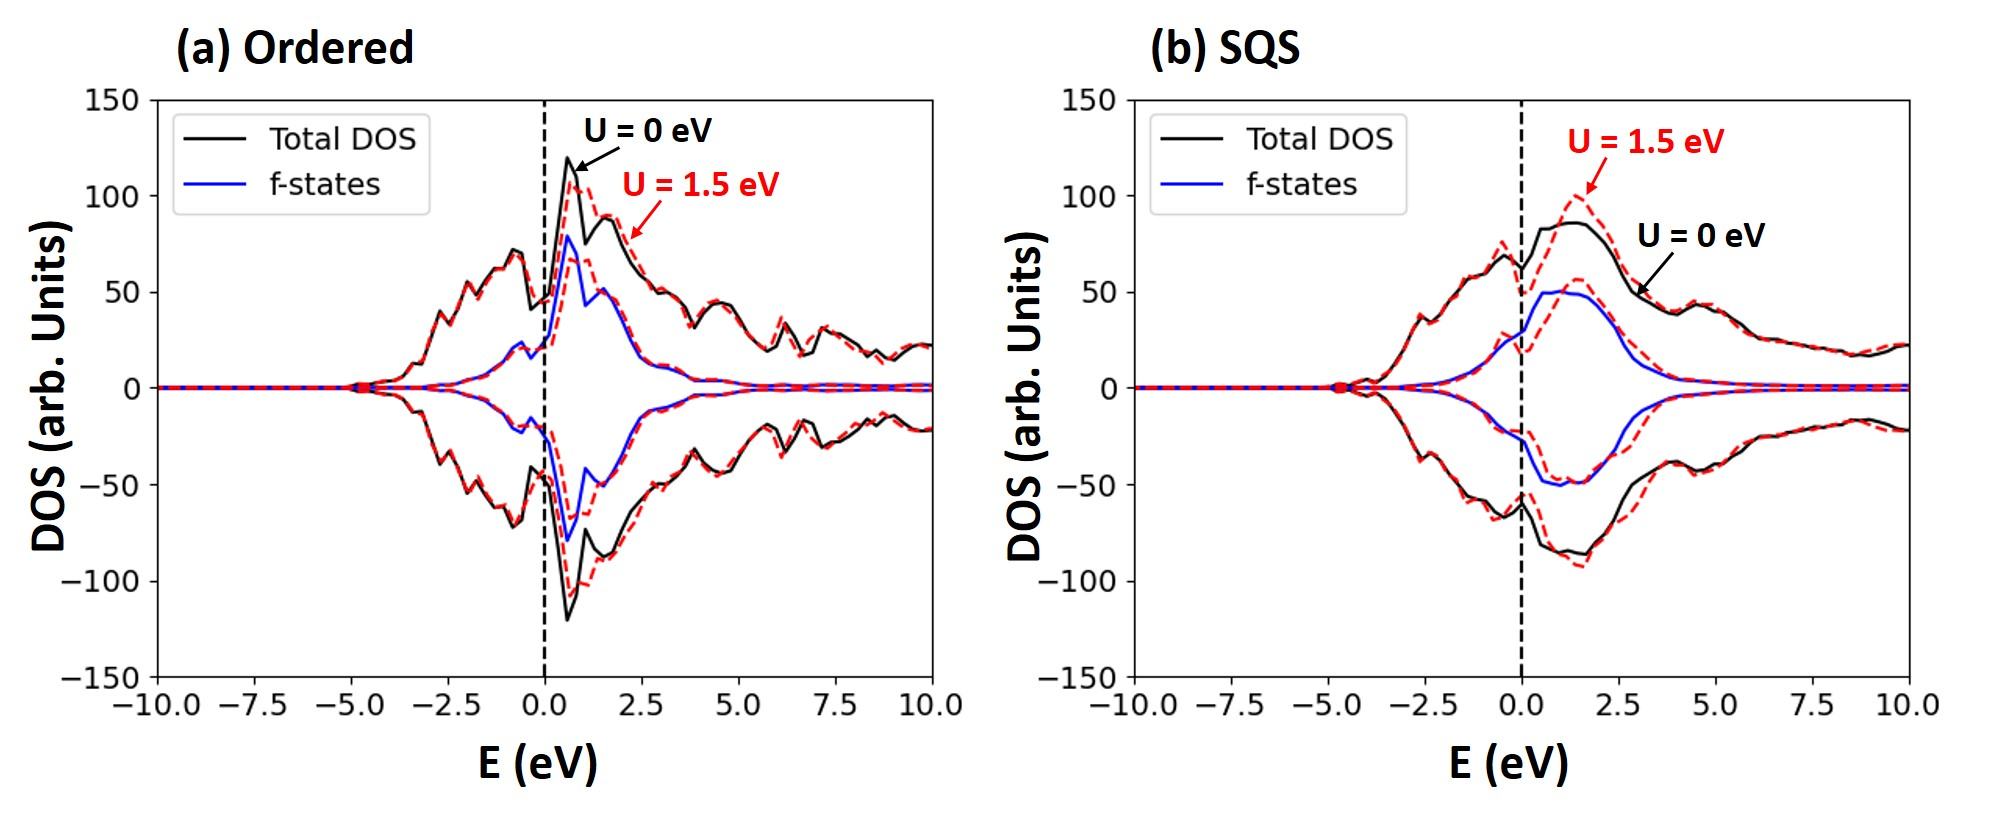
\includegraphics[scale=0.45]{DOS.jpg}
    \caption{The total and partial density of states of the uranium $f$-orbital using GGA (U = 0) (solid) and using GGA+U (U = 1.5 eV) (dashed) for (a) the ordered supercell, and (b) the SQS cell. }
    \label{fig:5}
\end{figure}

\section{Discussion}

Finally, we emphasize that the usage of Hubbard U to fit the formation enthalpy of $\delta$-UZr$_2$ is unjustifiable and not recommended. It not only overestimates the volume, but it also introduces unphysical magnetism. Reasonable equilibrium volumes, thermal expansion, heat capacities, elastic constants, and magnetic properties are obtained for a pure GGA treatment of this intermetallic phase. This conclusion agrees with the letter by Soderlind et al. \cite{soderlind_electron_2014} suggesting a weak electron correlation in U metal and the U-Zr system in their study on the $\gamma$ phase. Additionally, it appears that either ordered or SQS supercells with AFM ordering are appropriate to describe $\delta$-UZr$_2$. While the volume more closely matches experimental results for the SQS cell, there is a negligible difference in the heat capacity and the induced magnetism. Additional insight can be gained by utilizing ordered supercells, specifically directionally dependent phenomena such as elastic constants and anisotropic lattice expansion. 

\FloatBarrier
\section{Conclusions}
In this work, we investigated the structure and thermophysical properties of $\delta$-UZr$_2$ using DFT calculations. Chemically ordered supercells and SQS cells were considered in this study to simulate the partially ordered $\delta$-UZr$_2$. We employed different magnetic states to model the true paramagnetism of this phase. For the first time, we found that antiferromagnetic ordering is the ground state for UZr$_2$ according to GGA and GGA+U. We were able to overcome the ferromagnetic local minimum that was reported in previous DFT studies due to equilibration at a finite temperature of 100 K using AIMD. This was also the first study that utilized AIMD methods to investigate $\delta$-UZr$_2$. After exploring the magnetic behavior in the UZr$_2$ system, we conclude that pure GGA is more suitable for describing the $\delta$ phase of the U-Zr system. Our approach of using pure GGA (U=0) supported by AIMD equilibration eliminates the empiricism associated with choosing a Hubbard U value. This approach results in a ground-state solution with weak antiferromagnetism that mimics paramagnetism. It also reproduces atomic volume, thermal expansion, and heat capacities that are consistent with experimental measurements. Further experimental measurements, especially on the enthalpy of formation, are warranted to validate the presented results.  

\FloatBarrier
%\section{Declaration of Competing Interests}
%The authors declare that they have no known competing interests.

\FloatBarrier
\section{Acknowledgments}

This work was partially supported by grants from the U.S. Department of Energy, Office of Nuclear Energy (DOE-NE) (DE-NE0009271, Project 22-26632). This research made use of the resources of the High-Performance Computing Center at Idaho National Laboratory, which is supported by the Office of Nuclear Energy of the U.S. Department of Energy and the Nuclear Science User Facilities under Contract No. DE-AC07-05ID14517.

%% The Appendices part is started with the command \appendix;
%% appendix sections are then done as normal sections
%\appendix

%\section{Sample Appendix Section}
%\label{sec:sample:appendix}


%% If you have bibdatabase file and want bibtex to generate the
%% bibitems, please use
%%
 \bibliographystyle{elsarticle-num} 
 \bibliography{delta_UZr2}

%% else use the following coding to input the bibitems directly in the
%% TeX file.

% \begin{thebibliography}{00}

% %% \bibitem{label}
% %% Text of bibliographic item

% \bibitem{}

% \end{thebibliography}
\end{document}
\endinput
%%
%% End of file `elsarticle-template-num.tex'.
